\section{Derivazione del modello}
Consideriamo una corda di lunghezza $L$ e densit\`a lineare di massa $\rho_0$
costante a riposo.\\
Sia $t≥ 0$ il tempo, $x \in [0,L]$ la posizione in orizzontale,
$u(t,x)$ lo spostamento in verticale dalla posizione di riposo durante la
vibrazione della corda che pensiamo perfettamente flessibile.
Lo spostamento \`e assunto solo verticale e con vibrazioni di piccola ampiezza
rispetto ad L. Si trascurano gli attriti.\\
Si parte dalla conservazione della massa. Indichiamo con $\rho (t,x)$ la
densit\`a
lineare di massa al tempo $t$ nella posizione $x$. L'elemento di lunghezza al
tempo (fissato) $t$ \`e
\[
	ds=\sqrt{1+u_x^2} dx
\]
visto che si ha a che fare con una curva cartesiana
\[
	\left\{
	\begin{array}{ll}
		\begin{array}{l}
			x=x \\
			u=u(t,x)
		\end{array}
	& 0 ≤ x ≤ L
	\end{array}
	\right.
\]
nel piano $x,u$
\begin{figure}[H]
	\centering
	\includegraphics[width=0.6\textwidth]{wave_plane.pdf}
	\caption{$u(t,x)$ con $t$ fissato.}
	\label{wave_plane}
\end{figure}
La conservazione della massa si scrive
\[
	\rho ds= \rho_0 dx
\]
quindi
\[
	\rho \sqrt{1 + u_x^2}= \rho_0
\]
Ora imponiamo che le componenti orizzontali delle forze si bilancino, dato lo
spostamento solo verticale.
Assumiamo che l'unica forza non completamente verticale  applicata nei punti
della corda, sia la tensione, forza diretta tangenzialmente data la corda
perfettamente
flessibile.
Precisamente, il vettore tensione ${\bf T}(t,x)$ indica la forza che la porzione
di corda a distanza dal punto $(x, u(t,x))$ esercita sulla porzione a sinistra.
Evidentemente ${\bf -T}(t,x)$ \`e la forza che la porzione a sinistra esercita
su
quella a destra.
\begin{figure}[H]
	\centering
	\includegraphics[width=0.6\textwidth]{tension.pdf}
	\caption{Tensione sulla corda.}
	\label{tension}
\end{figure}
Indichiamo con $T(t,x)$ l'intensit\`a di ${\bf T}(t,x)$ e con $\alpha= \alpha
(t,x)$
l'inclinazione della corda rispetto alla posizione di riposo (asse $x$).
\[
	tg \alpha = u_x
\]
\begin{figure}[H]
	\centering
	\includegraphics[width=0.6\textwidth]{tension_alpha.pdf}
	\caption{Tensione sulla corda con $\alpha$ mostrato.}
	\label{tension_alpha}
\end{figure}
Il bilancio della componente orizzontale della tensione in un breve intervallo
$[x,x+\Delta x]$ impone
\[
	cos(\alpha + \pi)= - cos \alpha
\]
\begin{figure}[H]
	\centering
	\includegraphics[width=0.8\textwidth]{tension_dx.pdf}
	\caption{Tensione sulla corda tra due punti distanti $dx$.}
	\label{tension_dx}
\end{figure}
\[
	T(t, x + \Delta x) cos \; \alpha(t, x + \Delta x)-
	T(t,x)cos \; \alpha(t,x)=0
\]
Dividendo per $\Delta x$ e mandando $\Delta x \to 0$
\[
	\frac{\partial}{\partial x}[T(t,x) cos \; \alpha(t,x)]=0
\]
da cui
\[
	T(t,x) cos \; \alpha(t,x)= \tau
\]
con $\tau$ indipendente da $x$.
La componente orizzontale della tensione, detta trazione, non dipende dalla
posizione. Se assumiamo che la tensione sia di intensit\`a proporzionale
alla lunghezza della porzione di corda che la esercita, allora $\tau$ \`e
indipendente anche da $t$ visto che la lunghezza in orizzontale \`e costante
$L$.\\
Calcoliamo ora la componente verticale della tensione nel tratto di corda
corrispondente a $[x, x+ \Delta x]$. Tenendo conto di $sin(\alpha + \pi)= - sin
\alpha$ e di $T= \tau/cos\alpha$, essa vale
\[
	T(t,x+\Delta x)sin \, \alpha(t, x+ \Delta x) - T(t,x)sin \, \alpha
(t,x)=
\]
\[
	\tau[tg \, \alpha (t, x + \Delta x)- tg  \, \alpha(t,x)]=
\]
\[
	\tau[u_x \, \alpha (t, x + \Delta x)- u_x \alpha(t,x)]=
	\tau \int_x^{x+\Delta x} u_{xx}(t,y) dy
\]
Essendo una trazione, essa corrisponde ad una forza.\\
Denotiamo ora con $f(t,x)$ gli eventuali carichi totali per unit\`a di massa; se
il
peso non \`e trascurabile $f(t,x)= -g + F(t,x)$ dove $g$ \`e l'accelerazione
di gravit\`a ed $F$ corrisponde ad altri ulteriori carichi. Quindi
\[
	=\tau \int_x^{x+\Delta x} u_{xx}(t,y) dy +
	\int_x^{x+\Delta x} f(t,y) \rho (t,y) \sqrt{1+ u_x^2(t,y)} dy
\]
Per il principio fondamentale della dinamica, forza = massa $\cdot$
accelerazione rappresenta sempre una forza
\[
	\underbrace{\int_x^{x+\Delta x} u_{tt}(t,y) \rho (t,y) \sqrt{1+
u_x^2(t,y)} dy}_{
	\text{accelerazione $\cdot$ massa}}
\]
perci\`o
\begin{align*}
	\int_x^{x+\Delta x} u_{tt}(t,y) \rho (t,y) \sqrt{1+ u_x^2(t,y)} dy&= \\
	\tau \int_x^{x+\Delta x} u_{xx}(t,y) dy &+
	\int_x^{x+\Delta x} f(t,y) \rho (t,y) \sqrt{1+ u_x^2(t,y)} dy
\end{align*}
che pu\`o essere scritta
\[
	\int_x^{x+\Delta x}\rho_0 u_{tt}(t,y)  dy=
	\int_x^{x+\Delta x} \tau u_{xx}(t,y) dy +
	\int_x^{x+\Delta x} \rho_0 f(t,y)  dy
\]
\[
	\int_x^{x+\Delta x} \left[
	\rho_0 u_{tt} - \tau u_{xx}-  \rho_0 f
	\right]dy= 0
\]
Per l'arbitrariet\`a del tratto $[x, x+ \Delta x]$, deve essere
\[
	\rho_0 u_{tt} - \tau u_{xx}-  \rho_0 f
\]
Dividendo per $\rho_0$ ed indicando $c^2=\tau / \rho_0$ si ha l'equazione
\[
	u_{tt} - c^2 u_{xx} = f
\]
La costante $c$ ha la dimensione di una velocit\`a.
\section{Problemi ben posti}
Esistenza, unicit\`a e dipendenza continua dai dati si hanno imponendo le
condizioni iniziali
\[
\begin{array}{ll}
	u(0,x)=g(x) & \text{(spostamento iniziale)}\\
	u_t(0,x)=h(x) & \text{(velocit\`a iniziale)}
\end{array}
\]
e selezionando uno tra i seguenti tipi di condizioni agli estremi.
\subsubsection{Dirichlet}
\[
	u(t,0)=a(t), \;\;\; u(t,L)=b(t)
\]
Si prescrive lo spostamento agli estremi.
In particolare gli estremi sono fissati per $a(t)= b(t)=0$
\subsubsection{Neumann}
\[
	\tau u_x(t,0)=a(t), \;\;\; -\tau u_c (t,L)=b(t)
\]
Si prescrive la componente verticale della tensione agli estremi.
\subsection{Energia}
L'energia immagazzinata dalla corda \`e data dalla somma dell'energia cinetica
e dell'energia potenziale. L'energia cinetica, dato
\[
	dL=Fdx=madx=m\frac{dv}{dt}dx=mdv\frac{dx}{dt}=mvdv
	\follows
	\int_0^t dL= m \int_0^t vdv
\]
\[
	L=\frac{1}{2}mv^2
\]
perci\`o
\[
	E_{cin}(t)= \frac{1}{2}\int_0^L \rho_0 u^2_t(t,x)dx
\]
L'energia potenziale vale il lavoro della trazione.
Calcoliamo l'allungamento per un tratto di corda $\Delta x$ a riposo. Vale
\[
	\int_x^{x + \Delta x} \sqrt{1+ u^2_x} dy - \Delta x=
	\int_x^{x + \Delta x} \left( \sqrt{1+ u^2_x}-1 \right) dy
\]
L'approssimazione lineare di $\sqrt{1+y}-1$ \`e $\frac{1}{2}y$ per $y \to 0$,
quindi l'approssimazione al primo ordine dell'allungamento \`e
\[
	\frac{1}{2} u^2_x \Delta x
\]
e l'energia potenziale vale
\[
	E_{pot}(t)= \frac{1}{2} \int_0^L \tau u^2_x (t,x)dx
\]
e l'energia totale \`e data da
\[
	E(t)= \frac{1}{2}\int_0^L \left[
	\rho_0 u^2_t + \tau u_x^2
	\right] dx
\]
Calcoliamo la variazione dell'energia:
\[
	E'(t)= \int_0^L \left[
	\rho_0 u_t u_{tt} + \tau u_x u_{xt}
	\right] dx
\]
Integriamo per parti il termine corrispondente all'energia potenziale
\[
	\int_0^L u_x u_{tx}dx=
	\left[ u_x u_t \right]_0^L -
	\int_0^L u_t u_{xx} dx
\]
avendo considerato continue le derivate e quindi lecito applicare il
teorema di Schwartz per invertire l'ordine di integrazione. Quindi
\[
	\int_0^L u_x u_{tx}dx=
	\underbracket{\left[ u_x(t,L) u_t(t,L) -  u_x(t,0) u_t(t,0) \right]}_{
	G(t)} -
	\int_0^L u_t u_{xx} dx
\]
Dunque
\[
	E'(t)= \int_0^L u_t (\rho_0 u_{tt} - \tau u_{xx})dx + \tau G(t)
\]
\[
	= \int_0^L u_t f dx + \tau G(t)
\]
tenuto conto dell'equazione $\rho_0 u_{tt} - \tau u_{xx}= f$.\\
In particolare, per $f=0$ (assenza di carichi) e per $G=0$ si ha $E'(t)=0$
da cui
\[
	E(t)= \text{costante}
\]
cio\`e l'energia \`e conservata.\\
$G=0$ si realizza con gli estremi fissati
\[
	u(t,0)=u(t,L)=0
\]
in quanto
\[
	u_t(t,0)=u_t(t,L)=0
\]
o con tensione verticale nulla agli estremi
\[
	u_x(t,0)=u_x(t,L)=0
\]
L'energia conservata \`e quella iniziale
\[
	E(t)=E(0)=\frac{1}{2}\int_0^L
	\left[
	\rho_0 u_t^2 (0,x) + \tau u^2_x (0,x)
	\right]dx
\]
\[
	=\frac{1}{2}\int_0^L
	\left[
	\rho_0 h^2(x) + \tau g'\,^2(x)
	\right]dx
\]
\subsection{Unicit\`a tramite l'energia}
Siano $u_1$, $u_2$ due soluzioni del problema di Dirichlet
\[
	\left\{
	\begin{array}{l}
		u_{tt} - c^2 u_{xx}= f \\
		u(0,x)=g(x) \\
		u_t(0,x)= h(x)\\
		u(t,0)=a(t), \;\;\; u(t,L)=b(t)
	\end{array}
	\right.
\]
la differenza $w=u_1-u_2$ risolve il problema
\[
	\left\{
	\begin{array}{l}
		w_{tt} - c^2 w_{xx}= f \\
		w(0,x)=0 \\
		w_t(0,x)= 0\\
		w(t,0)=0, \;\;\; w(t,L)=0
	\end{array}
	\right.
\]
L'equazione per $w$ \`e omogenea con dati di Dirichlet nulli, quindi l'energia
si conserva e vale per ogni $t\geq 0$ l'energia iniziale.
Poich\'e i dati iniziali sono anch'essi nulli, l'energia iniziale \`e nulla.
In definitiva $E(t)=0$ cio\`e
\[
	\int_0^L [\rho_0 w^2_t + \tau w_x^2]=0
\]
da cui $w_t=0$ e $w_x=0$.\\
La funzione $w(t,x)$ \`e quindi costante in $(t,x)$, ed essendo $w=0$ per
$t=0$, si ha
\[
	w(t,x)=0 \;\;\; \text{per ogni }(t,x)
\]
Il problema di Dirichlet ha soluzione unica.\\
Stesse considerazioni per il problema di Neumann.
\subsection{Esistenza e regolarit\`a della soluzione}
Consideriamo la vibrazione di una corda fissata agli estremi e senza carichi
\[
	\left\{
	\begin{array}{l}
		u_{tt} - c^2 u_{xx}= 0 \\
		u(0,x)=g(x) \\
		u_t(0,x)= h(x)\\
		u(t,0)=0, \;\;\; u(t,L)=0
	\end{array}
	\right.
\]
Cominciamo nel cercare soluzioni di
\[
	\left\{
	\begin{array}{l}
		u_{tt} - c^2 u_{xx}= 0 \\
		u(t,0)=0, \;\;\; u(t,L)=0
	\end{array}
	\right.
\]
con il metodo della separazione delle variabili imponendo
\[
	u(t,x)=v(t)w(x)
\]
\[
	w(0)=w(L)=0
\]
si ha
\[
	v''(t)w(x)=c^2w''(x)v(t)
\]
da cui
\[
	\frac{1}{c^2} \frac{v''(t)}{v(t)}= \frac{w''(x)}{w(x)}
\]
che si pu\`o realizzare solo con
\[
	\frac{1}{c^2} \frac{v''(t)}{v(t)}= k = \frac{w''(x)}{w(x)}
\]
con $k$ costante.\\
Consideriamo il problema
\[
	\left\{
	\begin{array}{l}
		w''= kw \\
		w(0)=0, \;\;\; w(L)=0
	\end{array}
	\right.
\]
Si hanno soluzioni non banali solo per $k= -\mu <0$
perch\'e per $k>0$ o $k=0$ le condizioni agli estremi portano a $w=0$,
essendo in tali casi
\[
	w=ae^{x\sqrt{k}} + b e^{-x \sqrt{k}} \;\;\; \text{o} \;\;\;
	w=ax+b
\]
il rispettivo integrale generale. In entrambi i casi
\[
	\begin{cases}
		w(0)=0 \\
		w(L)=0
	\end{cases}
	\follows
	\begin{cases}
		a=0 \\
		b=0
	\end{cases}
\]
Sia dunque $k=-\mu < 0$ che porta
\[
	w=a \, cos(\mu x) + b \, sin (\mu x)
\]
\[
	\begin{cases}
		w(0)=0 \\
		w(L)=0
	\end{cases}
	\follows
	\begin{cases}
		a=0 \\
		b \, sin (\mu L)=0
	\end{cases}
\]
Abbiamo soluzioni non nulle per
\[
	\mu= \mu_m = \frac{m \pi}{L} \;\;\; m=1,2,3, \ldots
\]
date da
\[
	w_m= b_m sin \left( \frac{m\pi}{L} x \right)
\]
Veniamo all'equazione
\[
	v''(t)= -\mu^2 t^2 v(t)
\]
per il fattore dipendente da $t$.
Le soluzioni sono date da
\[
	v= a \, cos(\mu c t) + b \, sin (\mu c t)
\]
Abbiamo cos\`i trovato le infinite soluzioni di
\[
	\left\{
	\begin{array}{l}
		u_{tt} - c^2 u_{xx}= 0 \\
		u(t,0)=0, \;\;\; u(t,L)=0
	\end{array}
	\right.
\]
date da
\[
	u_m=
	\underbrace{\left[ a_m \, cos \left( \mu c t \right)
	+ b_m \, sin \left( \mu c t \right) \right]}_{A_m(t)}
	sin \left( \frac{m\pi}{L} x \right)
\]
\[
	u_m=
	\left[ a_m \, cos \left( \frac{mc\pi}{L} t \right)
	+ b_m \, sin \left( \frac{mc\pi}{L} t \right) \right]
	 sin \left( \frac{m\pi}{L} x \right)
\]
con $m=1,2,3, \ldots$\\
Queste sono dette le ``vibrazioni possibili '' della corda fissata agli estremi.
La forma della vibrazione \`e prescritta dalla funzione $sin \left(
\frac{m\pi}{L} x \right)$
con ampiezza $A_m(t)$ di segno ed intensit\`a variabile nel tempo, ma periodica
di periodo minimo
\[
	T_m= 2\pi \frac{L}{mc \pi}= \frac{2L}{mc}
\]
e la relativa frequenza
\[
	\frac{1}{T_m}= m\frac{c}{2L}
\]
\begin{figure}[t]
	\centering
	\includegraphics[width=\textwidth]{wave_modes.pdf}
	\caption{Alcune ``istantanee'' delle prime tre vibrazioni possibili a
$t$ fissato.}
	\label{wave_modes}
\end{figure}
\noindent
Come si pu\`o notare in fig. \ref{wave_modes}, dopo un tempo $T=\frac{2L}{c}$
si rivedono le stesse configurazioni: per $u_1$ \`e la priva volta, per $u_2$ la
seconda e per $u_3$ la terza volta che si osserva lo stesso grafico.\\
La sovrapposizione di vibrazioni con frequenza tutte multiple della stessa
frequenza di base
\[
	\frac{1}{T_1}= \frac{c}{2L}
\]
produce il suono armonioso della corda vibrante. La sovrapposizione
\[
	u= \sum_{m=1}^{\infty} u_m =
	\sum_{m=1}^{\infty} \left[ a_m \, cos \left( \frac{mc\pi}{L} t \right)
	+ b_m \, sin \left( \frac{mc\pi}{L} t \right) \right]
	 sin \left( \frac{m\pi}{L} x \right)
\]
\`e la soluzione completa.\\
Si definiscono quindi le condizioni iniziali
\[
	\begin{array}{l}
	u(0,x)= g(x)
 	\\
	u_t(0,x)= h(x)
	\end{array}
\]
Ponendo $t=0$ nell'espressione di $u$ e $u_t$
\[
	g(x)= \sum_{m=1}^{\infty} a_m \, sin \left( \frac{m\pi}{L} x \right)
\]
e
\[
	h(x)= \sum_{m=1}^{\infty} \frac{mc\pi}{L} b_m \, sin \left(
	\frac{m\pi}{L} x \right)
\]
Si sviluppano i dati $g(x)$ e $h(x)$ in serie di sole sinusoidi per $x \in
[0,L]$ effettuando il prolungamento continuo dispari all'intervallo $[-L,L]$.\\
I coefficienti sono quindi forniti da
\[
	a_m= \frac{2}{L} \int_0^L g(x) sin \left( \frac{m\pi}{L} x \right) dx
\]
\[
	b_m= \frac{2}{mc \pi} \int_0^L h(x) sin \left( \frac{m\pi}{L} x \right)
dx
\]
La funzione $u(t,x)$ cos\`i trovata risolve il problema almeno nel senso delle
distribuzioni.
Affinch\'e sia una soluzione in senso usuale occorre che si possa derivare due
volte in $dt$ ed in $dx$ sotto il segno di serie.
Questo \`e possibile se se i coefficienti $a_m$ e $b_m$ decadono almeno come
$\/m^4$: derivando due volte si producono addendi con coefficienti $m^a_m$,
$m^2b_m$. La condizione
\[
	m^2|a_m|\leq \frac{cost.}{m^2}, \;\;\; m^2|b_m|\leq \frac{cost.}{m^2}
\]
\`e sufficiente per garantire poi la convergenza dominata della serie ottenuta
derivando termine a termine.\\
La regolarit\`a $C^4$ per $g$ e $C^3$ per $h$ ($b_m$ ha gi\`a un $m$ a
denominatore) \`e una ipotesi sufficiente.\\
Osserviamo una diversit\`a fondamentale con l'equazione della diffusione. Per
questa ultima, qualunque sia la regolarit\`a del dato iniziale, i coefficienti
di Fourier della soluzione per $t>0$ decadono come $e^{-m^2 \pi^2 Dt/L}$ cio\`e
come $e^{-\alpha m^2}$ per $m \to +\infty$.
La soluzione ha in quel caso tutte le derivate in $dt$ e in $dx$ per $t>0$.
\`E questo l'effetto regolarizzante della diffusione, assente per l'equazione
della corda vibrante. Ora la soluzione \`e $C^k$ se i dati sono $g \in C^{k+2}$
e $h \in C^{k+1}$, $k\geq 2$. La regolarit\`a dei dati fornisce la regolarit\`a
della soluzione.\\
Non abbiamo ora soluzioni stazionare n\'e regime transitorio. In assenza di
attrito, la corda vibra all'infinito con una sovrapposizione di vibrazioni
periodiche stabilite dai dati iniziali.
\subsection{Dipendenza continua dai dati}
Indichiamo con $||u(t, \cdot)||_2$ la norma in $L^2$ della soluzione al tempo
$t$ fissato
\[
	||u(t, \cdot)||_2=
	\left(
	\int_0^L |u(t,x)|^2 dx
	\right)^1/2
\]
Per Parseval
